\section{Data Analysis}

% ------------ section structure -----------------
% (a) discuss binning and event selection, corrections 
% (b) discuss what beam spin asymmetries are 
% (c) describe the fitting procedure used 
% -----------------------------------------------

\subsection{Corrections, Event Selection, \& Binning}
For this analysis $ep \rightarrow e\pi^+N$ events are identified by directly identifying the scattered electron and positive pion, and inferring the presence of the neutron.  
\\
After the electron and pion have been identified, their momenta are corrected using momentum corrections developed for the E1-F dataset by Marco Mirazita \cite{mirazita}.  Time of flight corrections are also implemented based on work by Nathan Harrison \cite{harrison}, including removal of non-functional TOF paddles on a run-by-run basis.
\\
After the particle identification and kinematic correction, kinematic restrictions of $Q^{2} > 1.0$ and $W > 2.0$ are implemented to confine our measurement to the commonly accepted DIS region.  The rest of the final state can be calculated for each event simply by comparing initial and final state four-vectors.
\begin{equation}
	X^{\mu} = e'(k'^{\mu}) + \pi^{+}(h^{\mu}) - e(k^\mu) - p(P^\mu) 
\end{equation}  

The missing neutron can be inferred by asking that $M_X = \sqrt{X^{\mu}X_{\mu}} \approx M_{N}$, in particular it is required that $0.89 < M_{X} < 1.01$.  Events passing these criteria are considered to be the final event sample.     
\\
These events are binned in 15 bins (in the variable $\cos{\theta_h}$, the cosine of the polar angle between the virtual photon and the hadron) of variable size which are chosen based on the statistical content in each bin, and the acceptance in that bin.  The most extreme backward angle was not used due to a large acceptance hole in the central phi regions, shown in figure (put figure and reference).  The $\phi_h$ distributions are binned for fitting in 12 symmetric bins of width 30 degrees.  (Add figure which shows the binning drawn over the phi vs. theta histogram).      

\begin{figure}
  \begin{center}
    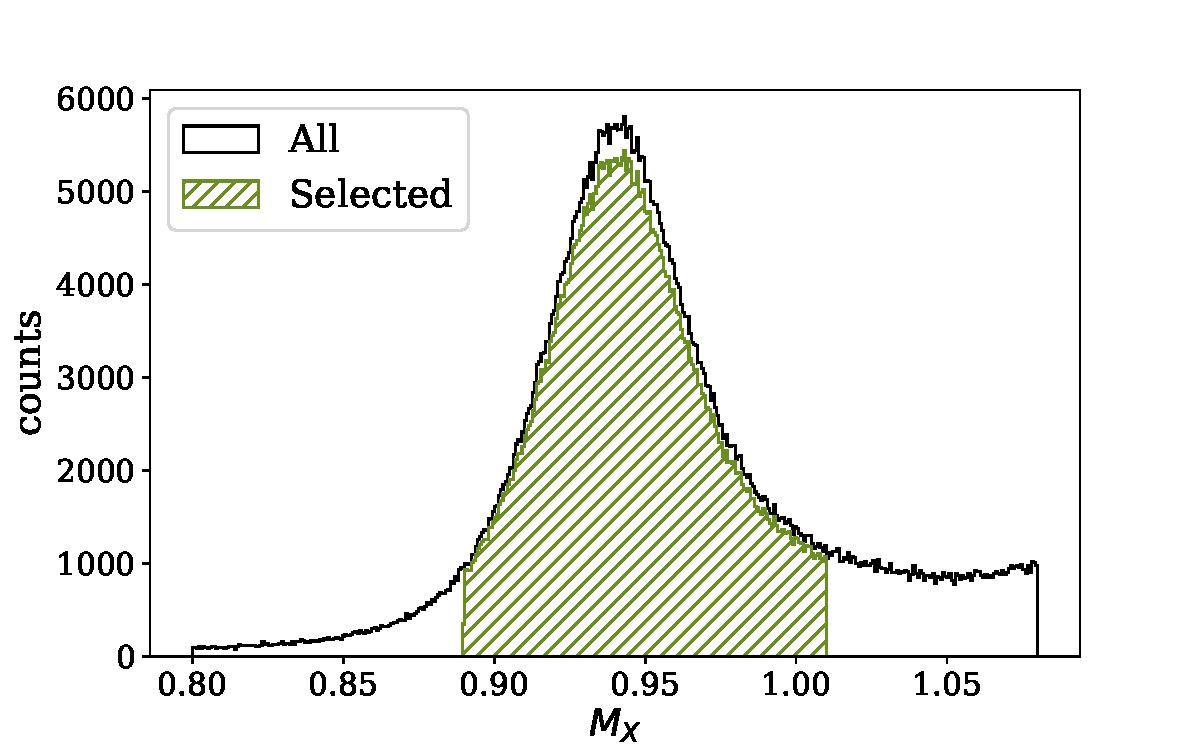
\includegraphics[width=\columnwidth]{image/missing_mass.pdf}
    \caption{Missing mass cut used to select neutrons.}
  \end{center}
\end{figure}

\begin{figure}
  \begin{center}
    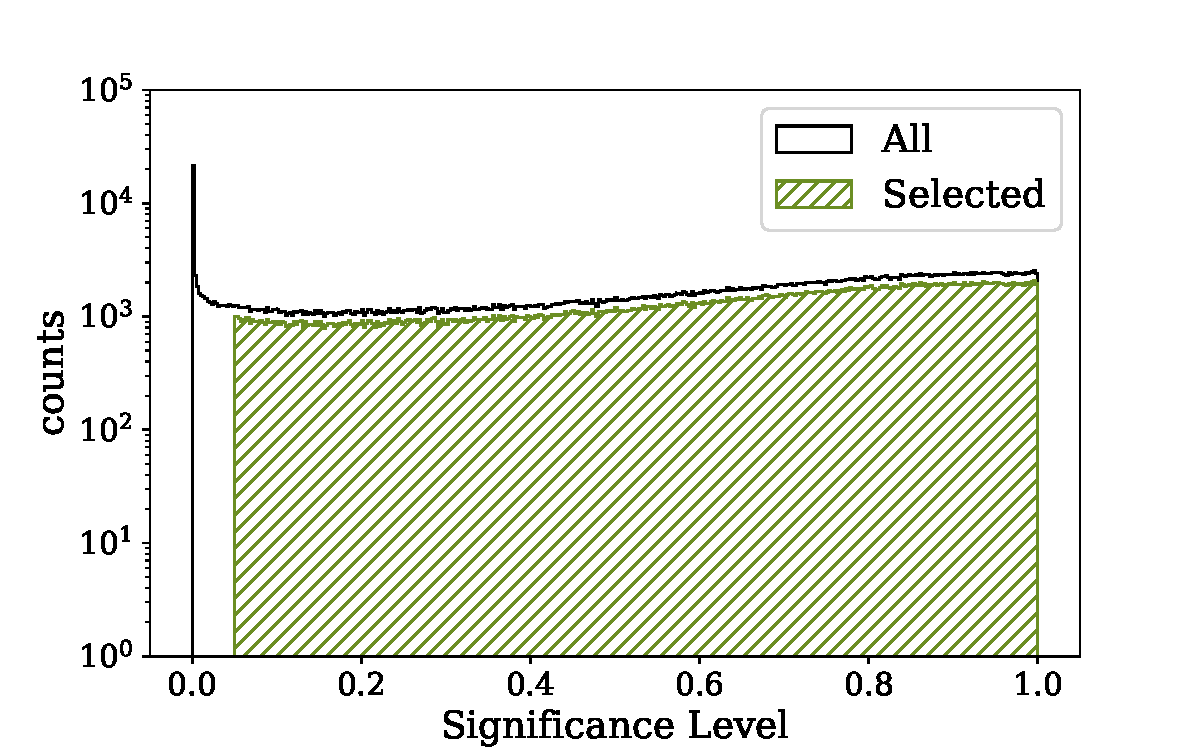
\includegraphics[width=\columnwidth]{image/significance.pdf}
    \caption{Significance level $\alpha$ before/after selection of final event sample.}
  \end{center}
\end{figure}

\begin{figure}
  \begin{center}
    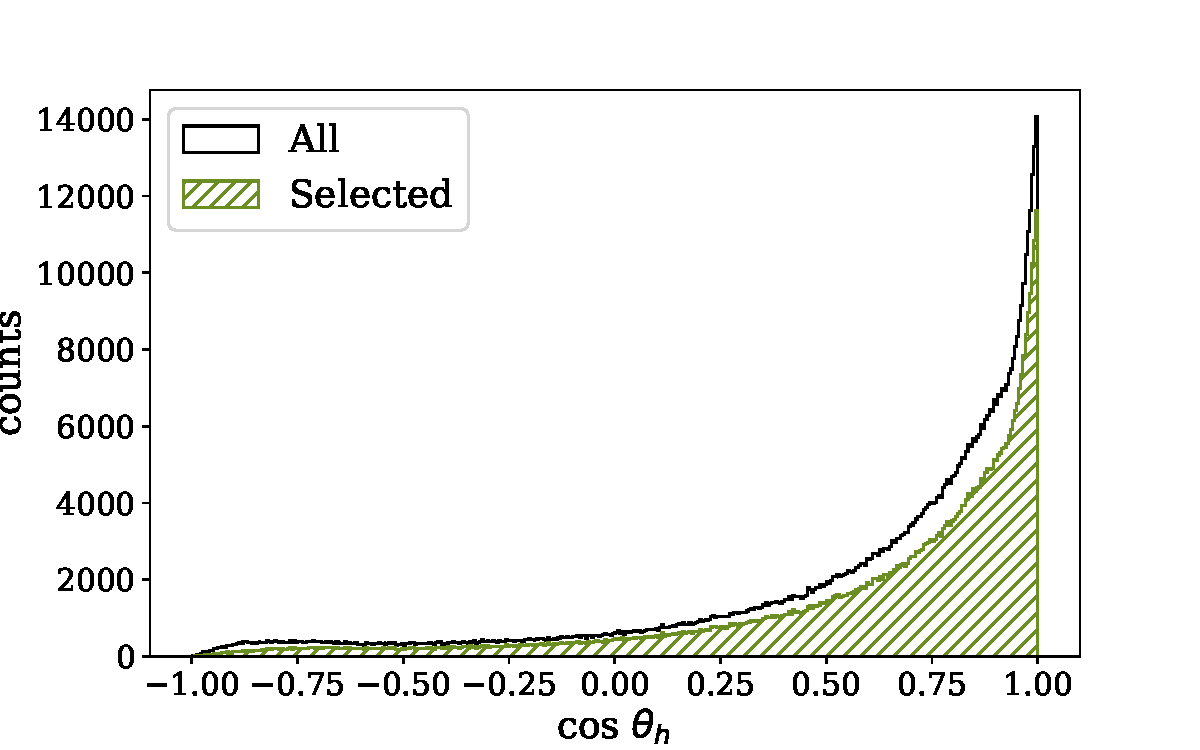
\includegraphics[width=\columnwidth]{image/cos_theta_h.pdf}
    \caption{Distribution of $cos \theta_h$ for positive pions before and after missing mass and pion siginificance cuts.}
  \end{center}
\end{figure}


\begin{figure}
  \begin{center}
    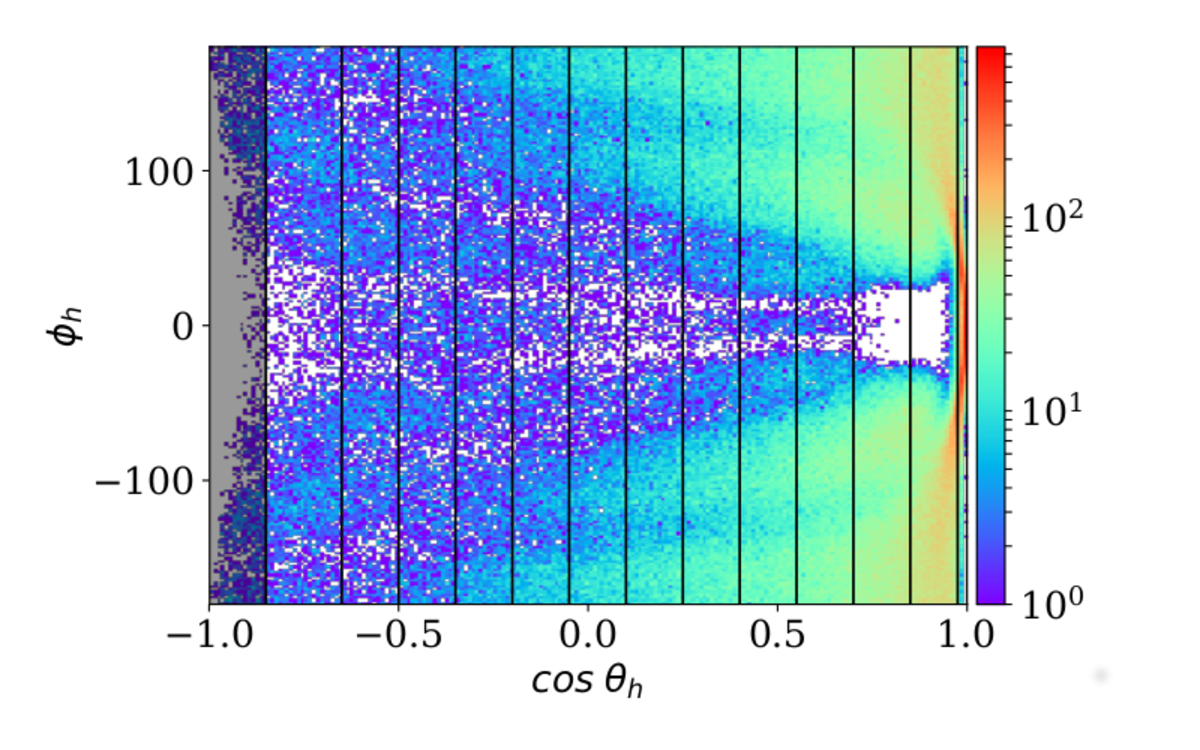
\includegraphics[width=\columnwidth]{image/cos_theta_h_phi_h_binned.pdf}
    \caption{Distribution of events in the center of mass of the $\gamma^* p^+$ system.  The extreme backward angles are removed for lack of data at central values of $\phi_h$.}
  \end{center}
\end{figure}

\subsection{Beam Spin Asymmetry}
Beam spin asymmetry (BSA) measurements are a go-to tool for Nuclear/Particle Physics, and will now be briefly introduced.  The cross section difference $d\sigma_{+} - d\sigma_{-}$, where the subscript refers to the lepton (electron) helicity projection along the beamline direction, is just the part of the cross section which depends on the electron spin state.  This quantity (interesting in itself) is not usually measured.  Instead the ratio,
\begin{equation}
	BSA = \frac{1}{P_e} \frac{d\sigma_{+} - d\sigma_{-}}{d\sigma_{+} + d\sigma_{-}} \approx \frac{1}{P_e} \frac{N_+ - N_-}{N_+ + N_-}
\end{equation}    
is presented, due to convenient cancellations in detector efficiency and acceptances in each cross section term.  Where the fractional polarization of the beam is denoted as $P_e$.  As mentioned in section 2, the beam spin is flipped at a rate of 33 Hz to minimize systematic errors arising due to differences in detector position and calibration.  
\\

\begin{figure}
  \begin{center}
    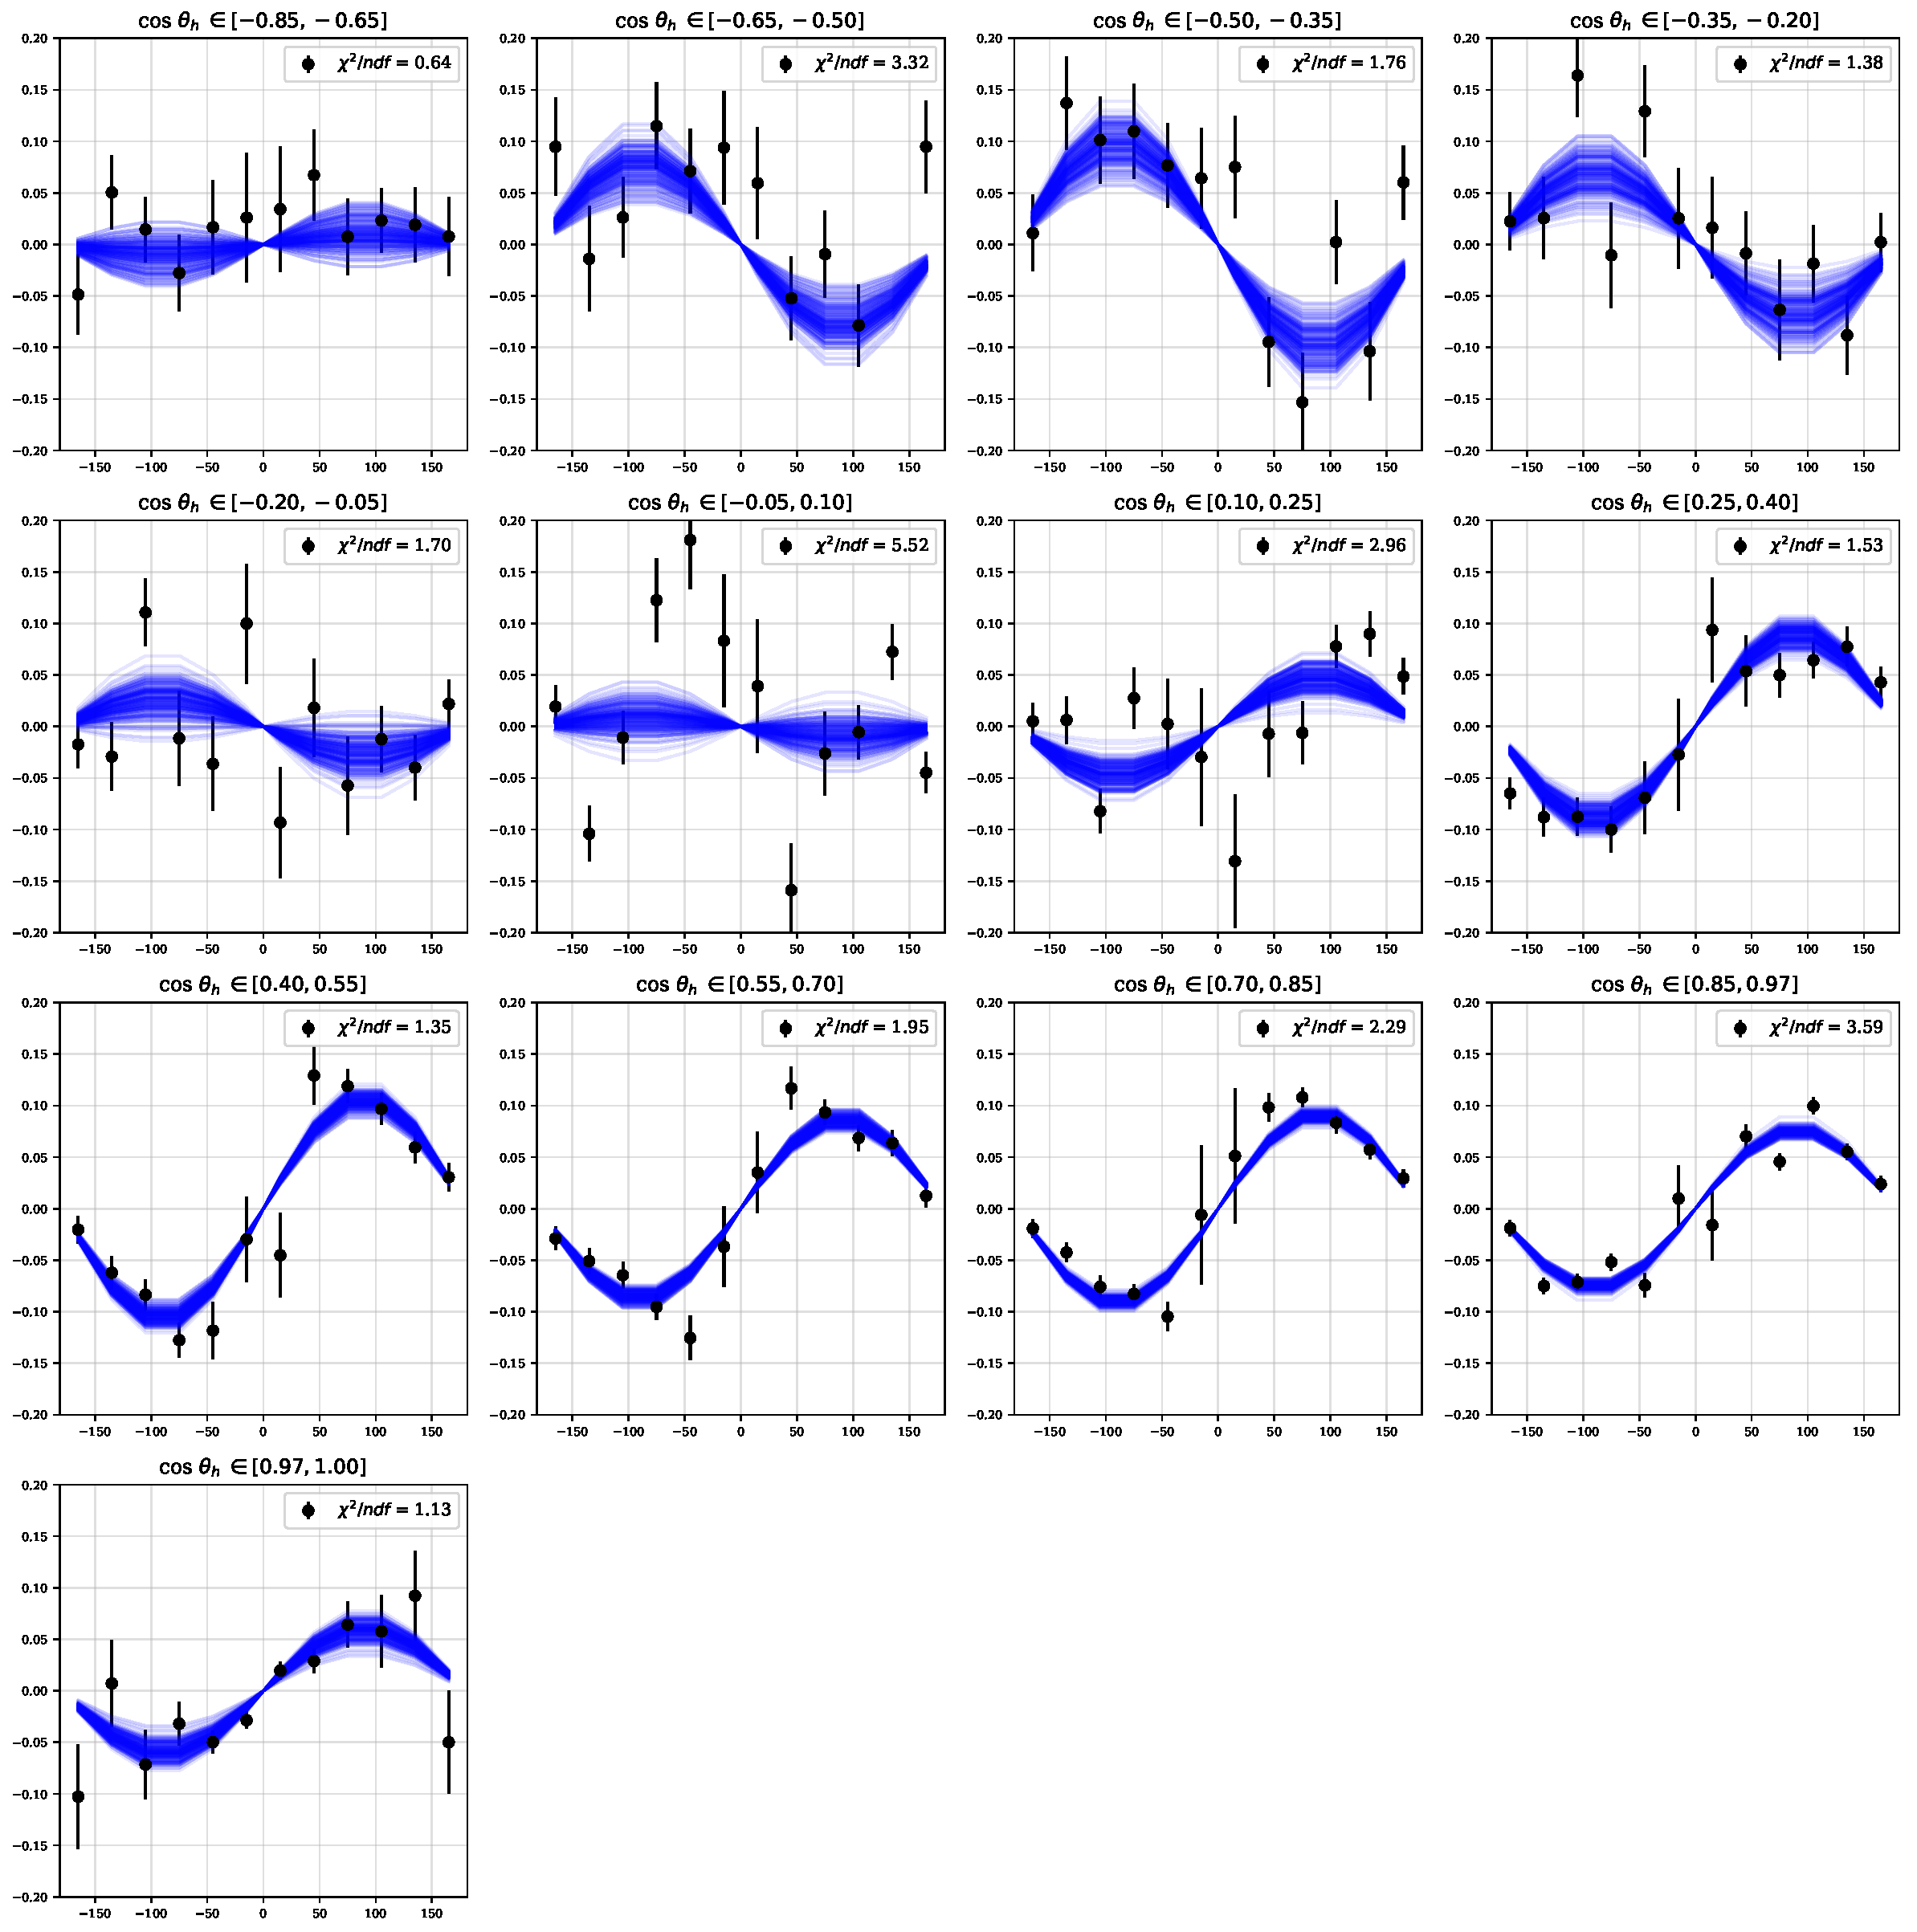
\includegraphics[width=\columnwidth]{image/default_phi_bootstraps.pdf}
    \caption{The BSA shown as a function of $\phi_h$ for different bins of $\cos \theta_h$.  Overlaid are the 200 bootstraps performed for each $\cos \theta_h$-bin.}
  \end{center}
\end{figure}

\subsection{Fitting Procedure}
The distributions for $\phi_h$ are binned and fit with the function $f(\phi_h) = A\sin{\phi_h}$ using $\chi^2$ minimization.  This is accomplished using the python implementation of gradient descent provided in \texttt{scipy.optimize.minimize}, which by default uses the \texttt{BFGS} method.  Parameter errors are calculated using two methods, first the common Hessian method, and second the bootstrap replica method.  These two methods are found to be consistent, and the parameter errors obtained by bootstrap methods are used throughout this report.   
\\    

\subsection{Systematic Errors}

% ------------ section structure -------------
% (a) summary of the systematic errors and their relative size 
% (b) description of different sources of error (fits, data inconsistany, cut choices)
% -------------------------------------------

The error on our measured values is considered in two categories.  First, statistical errors are calculated for the beam spin asymmetry measurement for every phi-bin.  During the fitting procedure, these statistical errors are mapped into errors on the fit parameters.  This first class of errors we consider as the statistcal error on the result.  Second, the authors consider all other possible sources of error which do not depend on statistical effects.  Those effects which have been identified are: \\


\begin{center}
\begin{tabular}{ | c || c |  }
 \hline
 Source & Relative Error\\
 \hline
 Cut: z-vertex                   & 0.0019\\
 Cut: \texttt{EC edep}           & 0.0027\\
 Cut: sampling fraction          & 0.0010\\
 Cut: $\theta_{CC}$ matching     & 0.0022\\
 Cut: pion significance $\alpha$ & 0.0049\\
 Beam Polarization               & 0.03  \\
 \hline
\end{tabular}
\end{center}

\subsubsection{Cut Variations}
In some cases, the direct variation of analyses parameters is the only way to try and understand the dependence of the result on the input parameters.  Ideally, the analysis result shouldn't vary outside of the errors which arise from statical fluctuations.    

\begin{figure}
  \begin{center}
    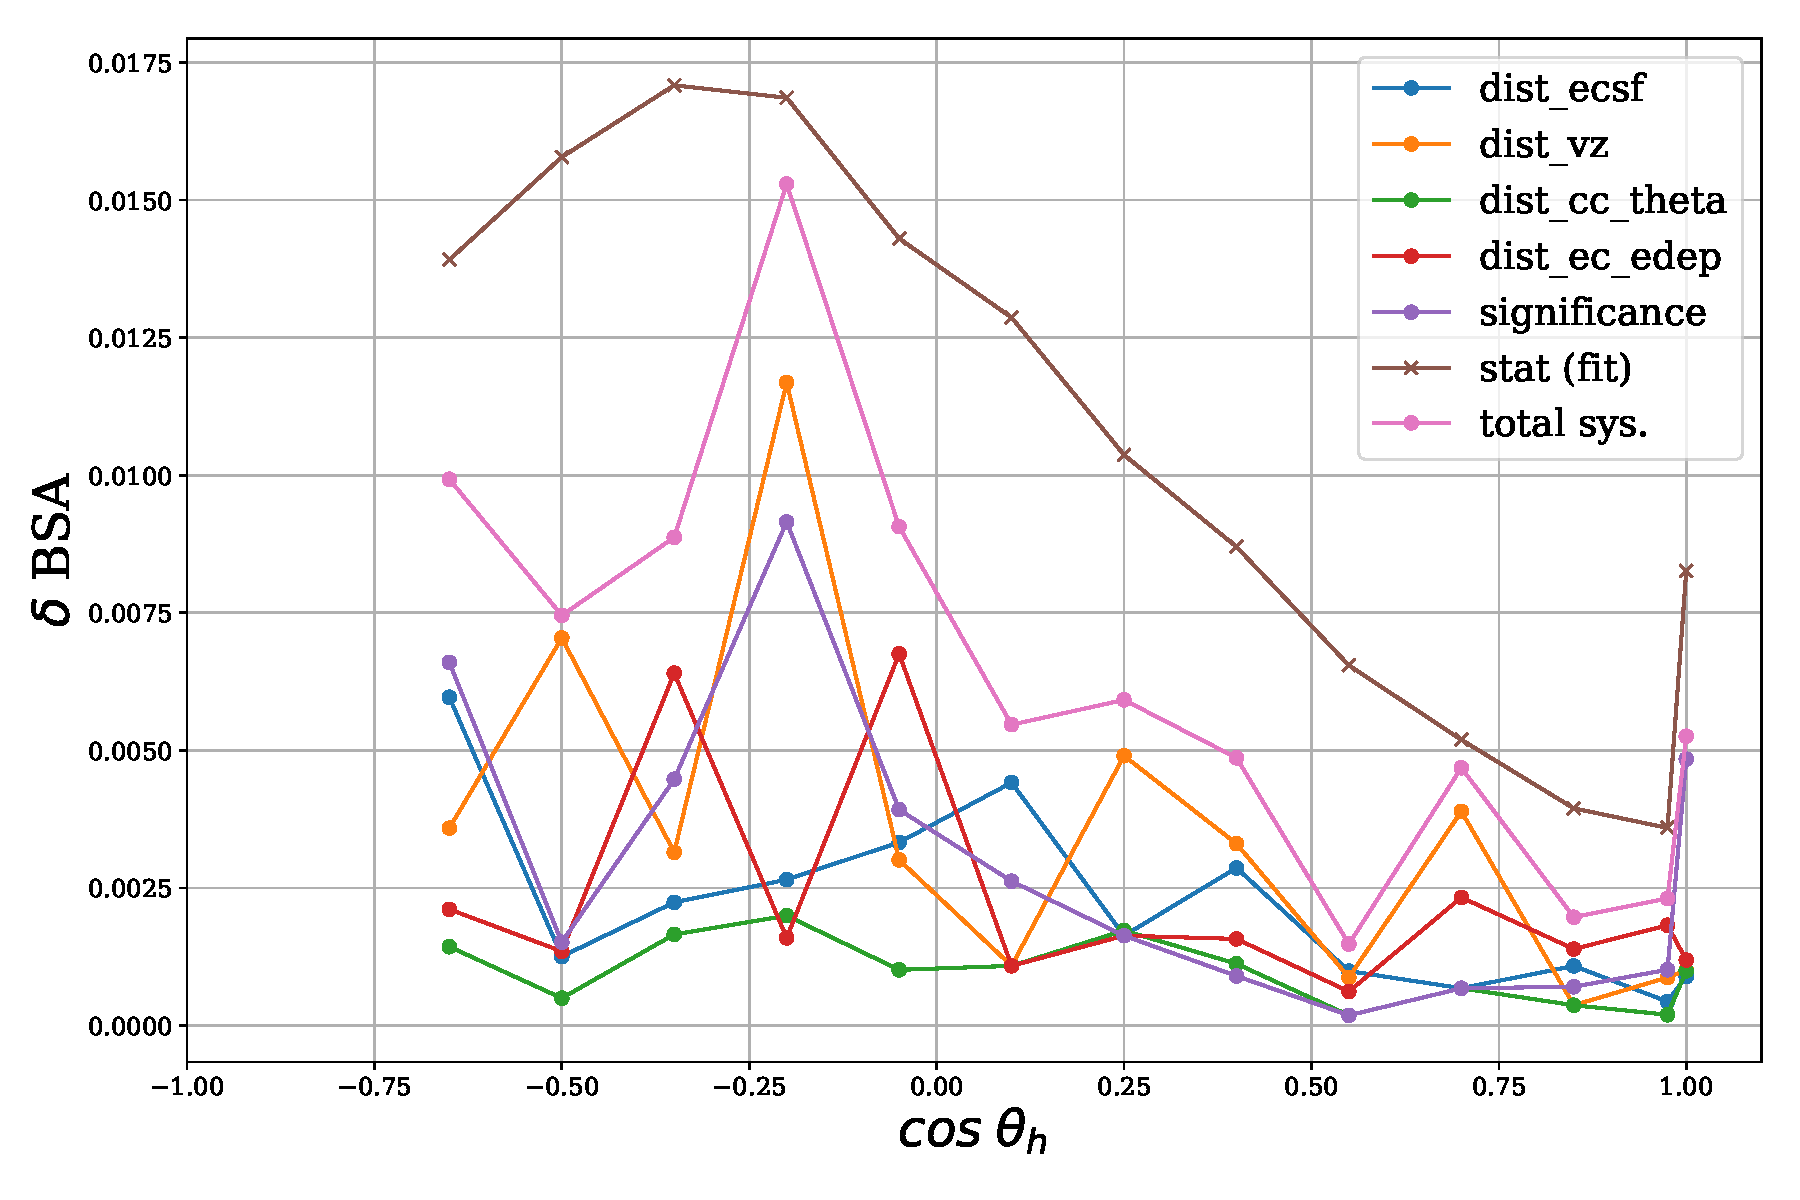
\includegraphics[width=\columnwidth]{image/systematics.pdf}
    \caption{The largest shift resulting from all variations of each analysis cut parameter.  Shown also is the statistical error.  All resulting cut variations remained withtin statistical error.}
  \end{center}
\end{figure}

\subsubsection{Random Subset/Helicity}

Two additional studies are performed which involve randomization of the input data in some way.  In the first study, the helicity of each event is assigned a random value of $\pm 1$.  This randomization destroys the correlation between beam spin and the $\phi_h$ distributions.  Therefore, one expects to find zero asymmetries as a result of this randomization.  In the second study, the full analysis is run on a subset of 80\% of the events in the full dataset.  This study is designed to identify if there is internal inconsistancy in the dataset.
\\

\begin{figure}
  \begin{center}
    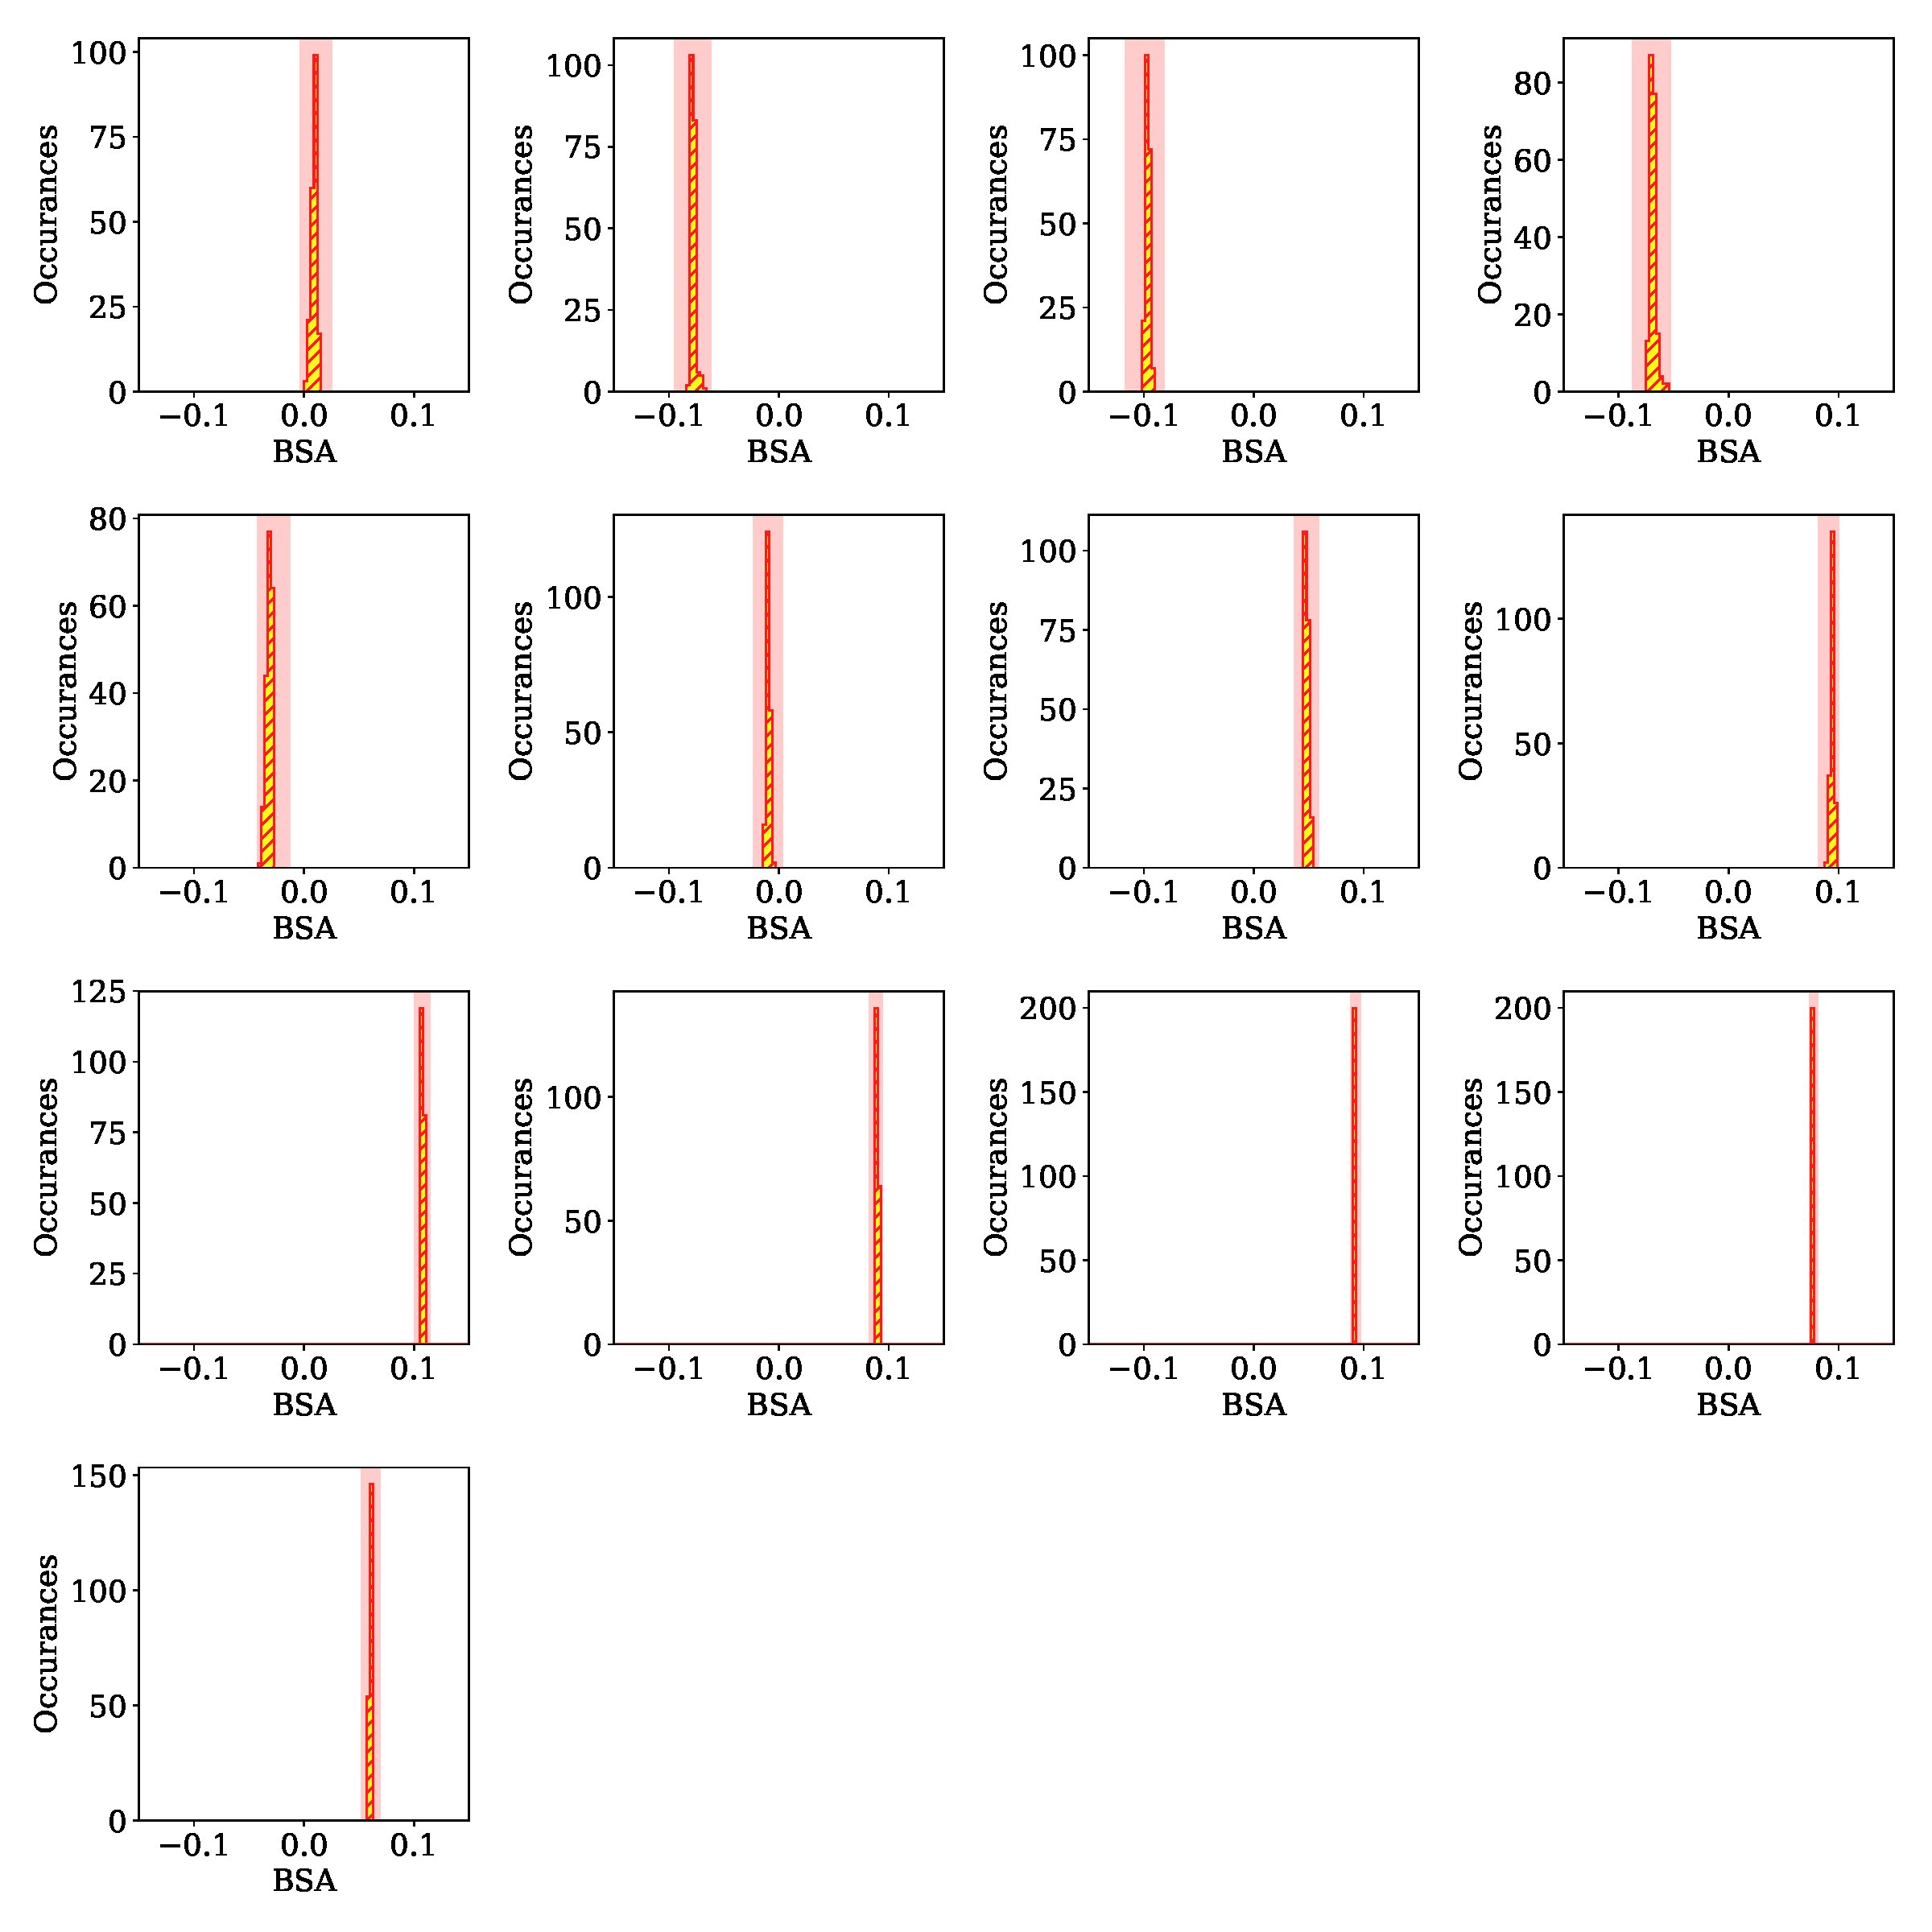
\includegraphics[width=\columnwidth]{image/subsets.pdf}
    \caption{Results for each bin of $\cos(\theta_h)$ calculated on 200 random subsets of 80\% of the entire dataset.  In the absence of internal inconsistency in the data, these results should be gaussianly distributed around the nominal result obtained with the entire dataset, which is shown with statistical error in red.}
  \end{center}
\end{figure}

\begin{figure}
  \begin{center}
    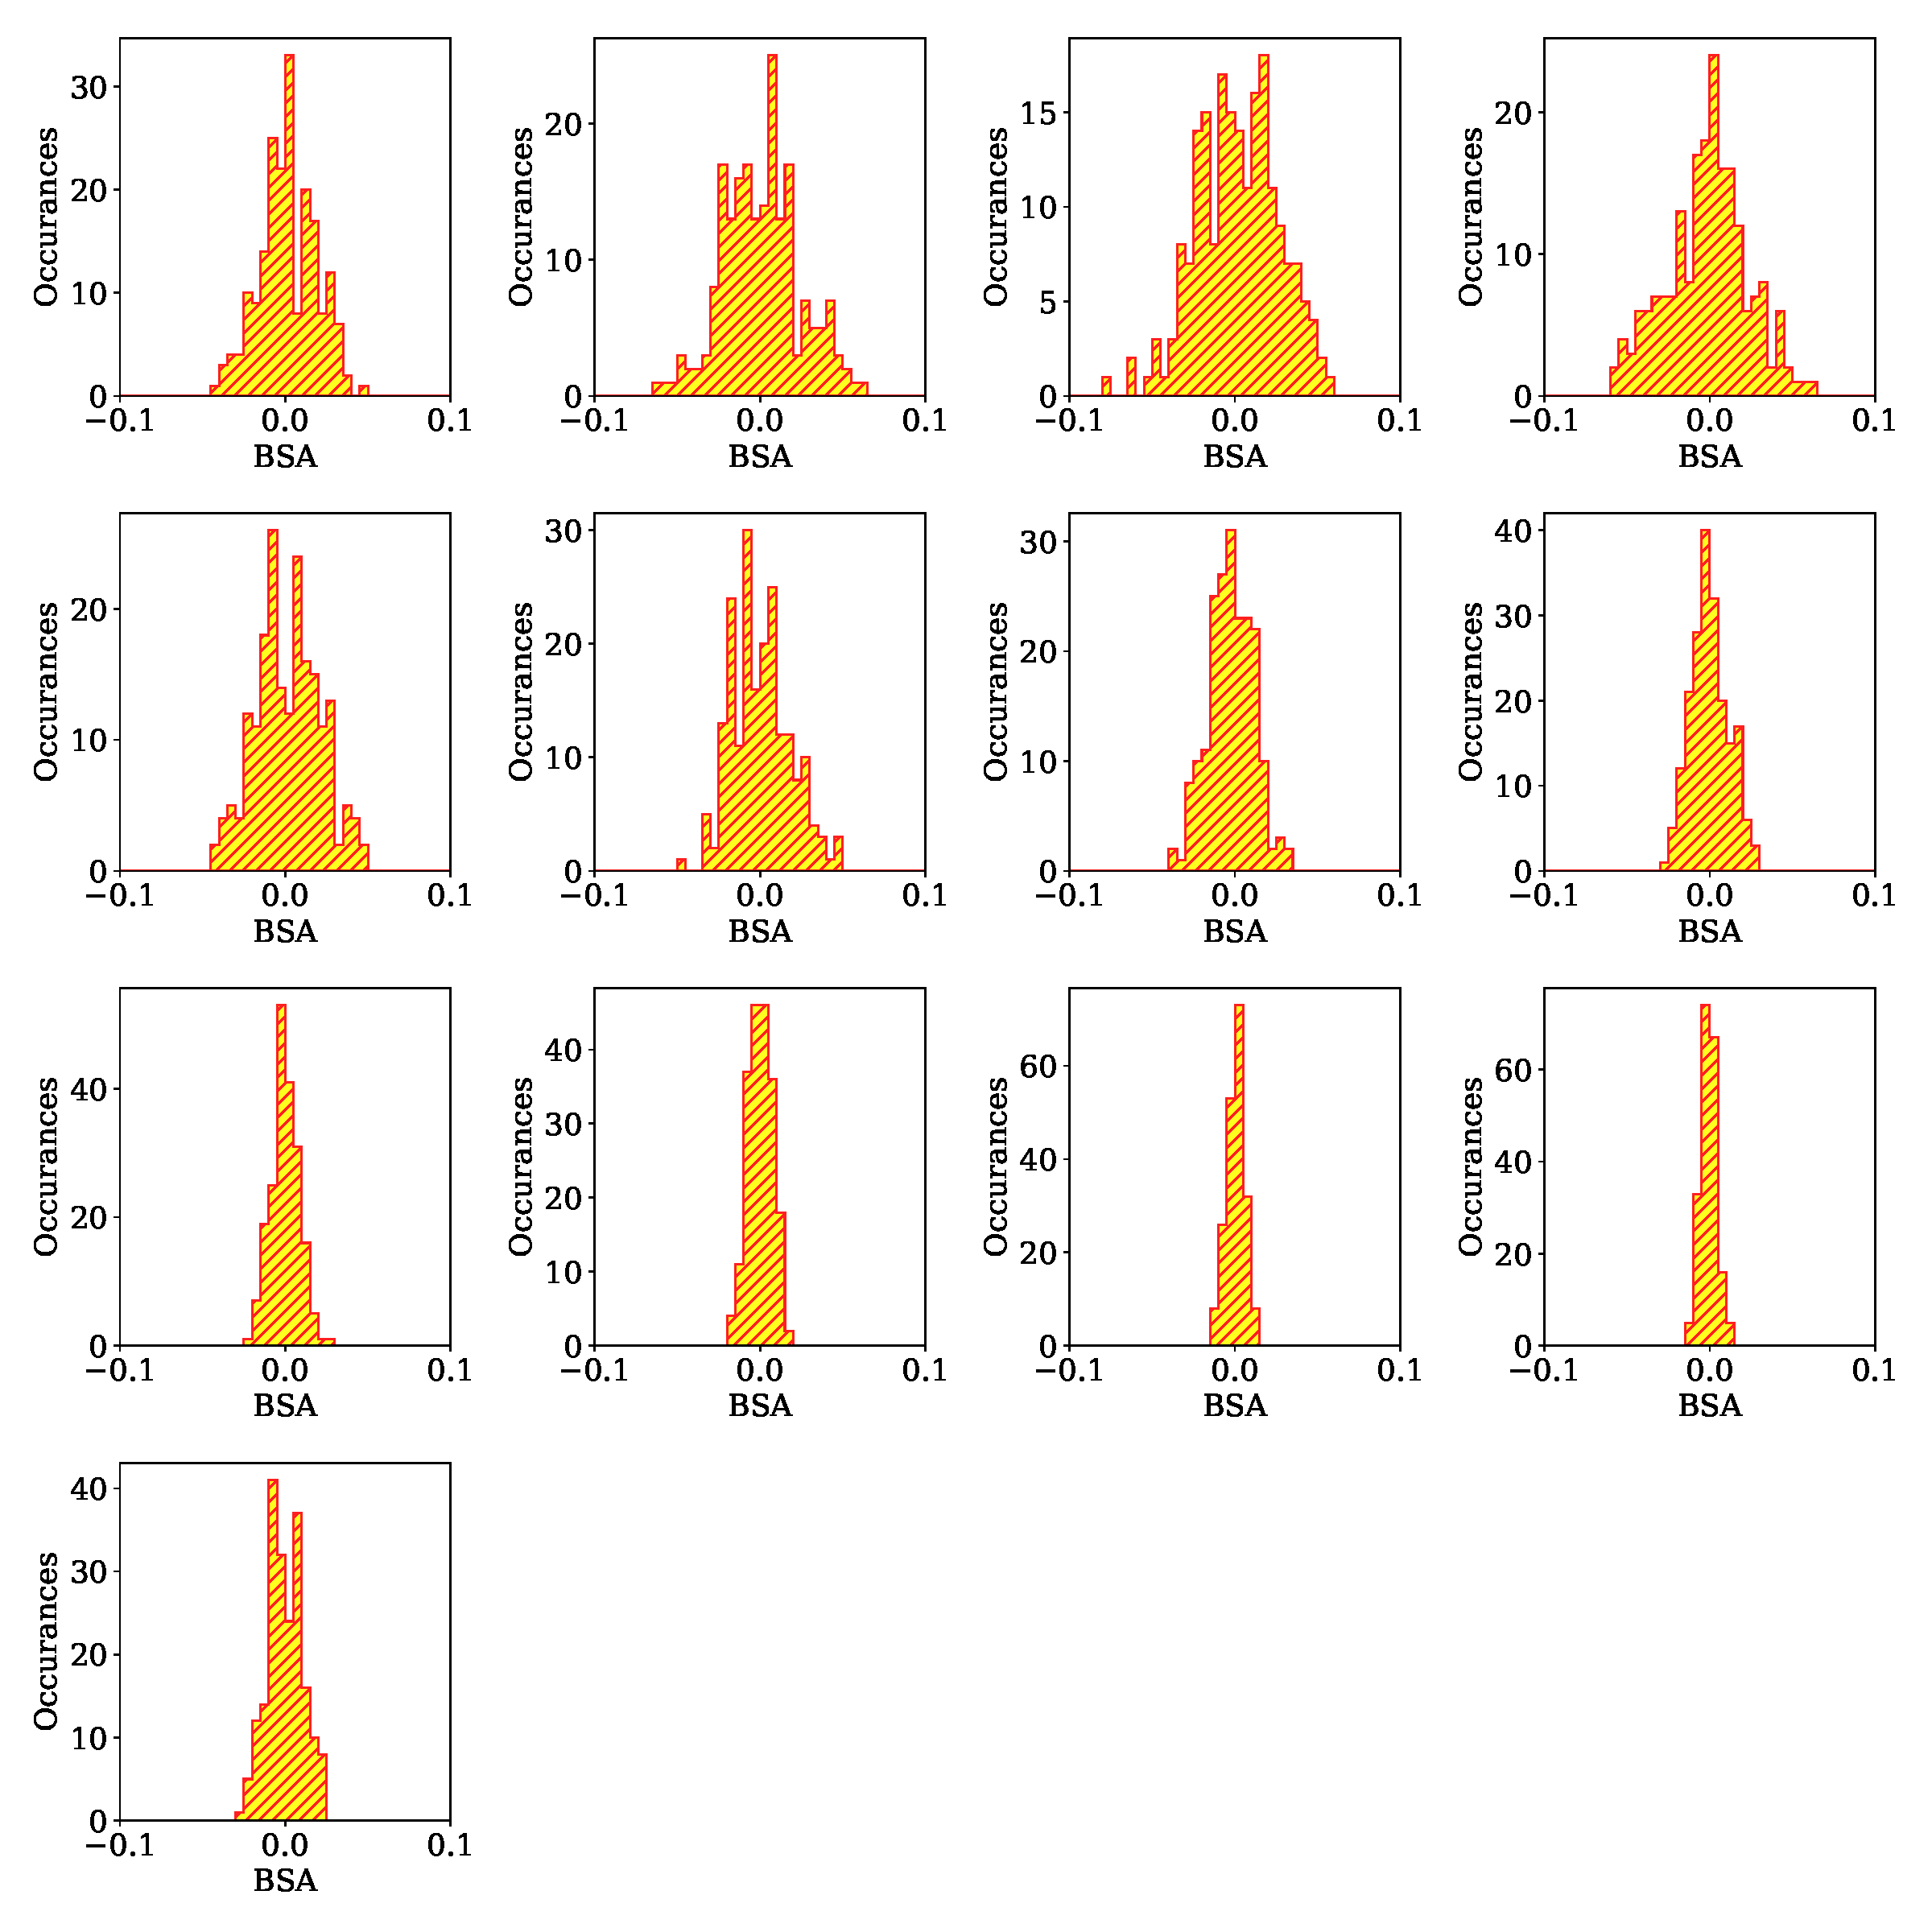
\includegraphics[width=\columnwidth]{image/helicity.pdf}
    \caption{Shown above are the results for randomizing the helicty for every event, and repeating the analysis 200 times.  This randomization destroys any correlation between the helicity states and the cross section, meaning that these results are expected to be zero (with larger fluctuation in lower statistics bins).}
  \end{center}
\end{figure}

